Our proposed method analyzes a video clip containing one person. The output is an estimate of the interview invitation variable, the big five OCEAN personality traits, the two mood primitives valence and arousal and lastly, the likeability variable. Only video features are used in our proposed method. This section will describe the main stages of our method, starting with describing our data-set and the process of annotating this data. Then the feature extraction and normalization processes are defined. Lastly, the classification methods are described. Figure \ref{fig:proposedmethod} shows the pipeline of our proposed method.

\begin{figure*}[h]
  \centering
  \includesvg[width=\textwidth]{Images/method_pipeline.svg}
  \caption{Flowchart of the proposed methodology.}
  \label{fig:proposedmethod}
\end{figure*}

\subsection{The Data Set}
\label{subsection:dataset}

For modeling and experimenting we relied on a publicly available data-set which contains 10,000 video clips with audio with an average duration of 15 seconds\footnote{The data-set can be found on http://chalearnlap.cvc.uab.es/dataset/24/description/}. The clips are collected from over 3000 videos available on YouTube. Figure \ref{fig:ssvideoclip} shows screenshots from four samples taken from the video clip data-set. The videos are annotated with the use of Amazon Mechanical Turk for apparent personality traits. These are the 5 OCEAN personality traits variables. Annotators saw a pair of video clips and were asked to rank the clips in order of which clip showed a higher score across the the 5 OCEAN personality trait variables. 

Furthermore, the videos are annotated for an additional variable, which is the interview variable. This variable measures whether a candidate should be invited for a job interview or not. Additionally these videos are annotated for ethnicity groups, age groups and gender (\cite{escalante2018explaining}). From this data-set of 10,000 videos the first 960 were selected for experimenting and further annotations of three more variables, namely, the valence, arousal and likeability variables. 


\begin{figure*}[h]
  \centering
  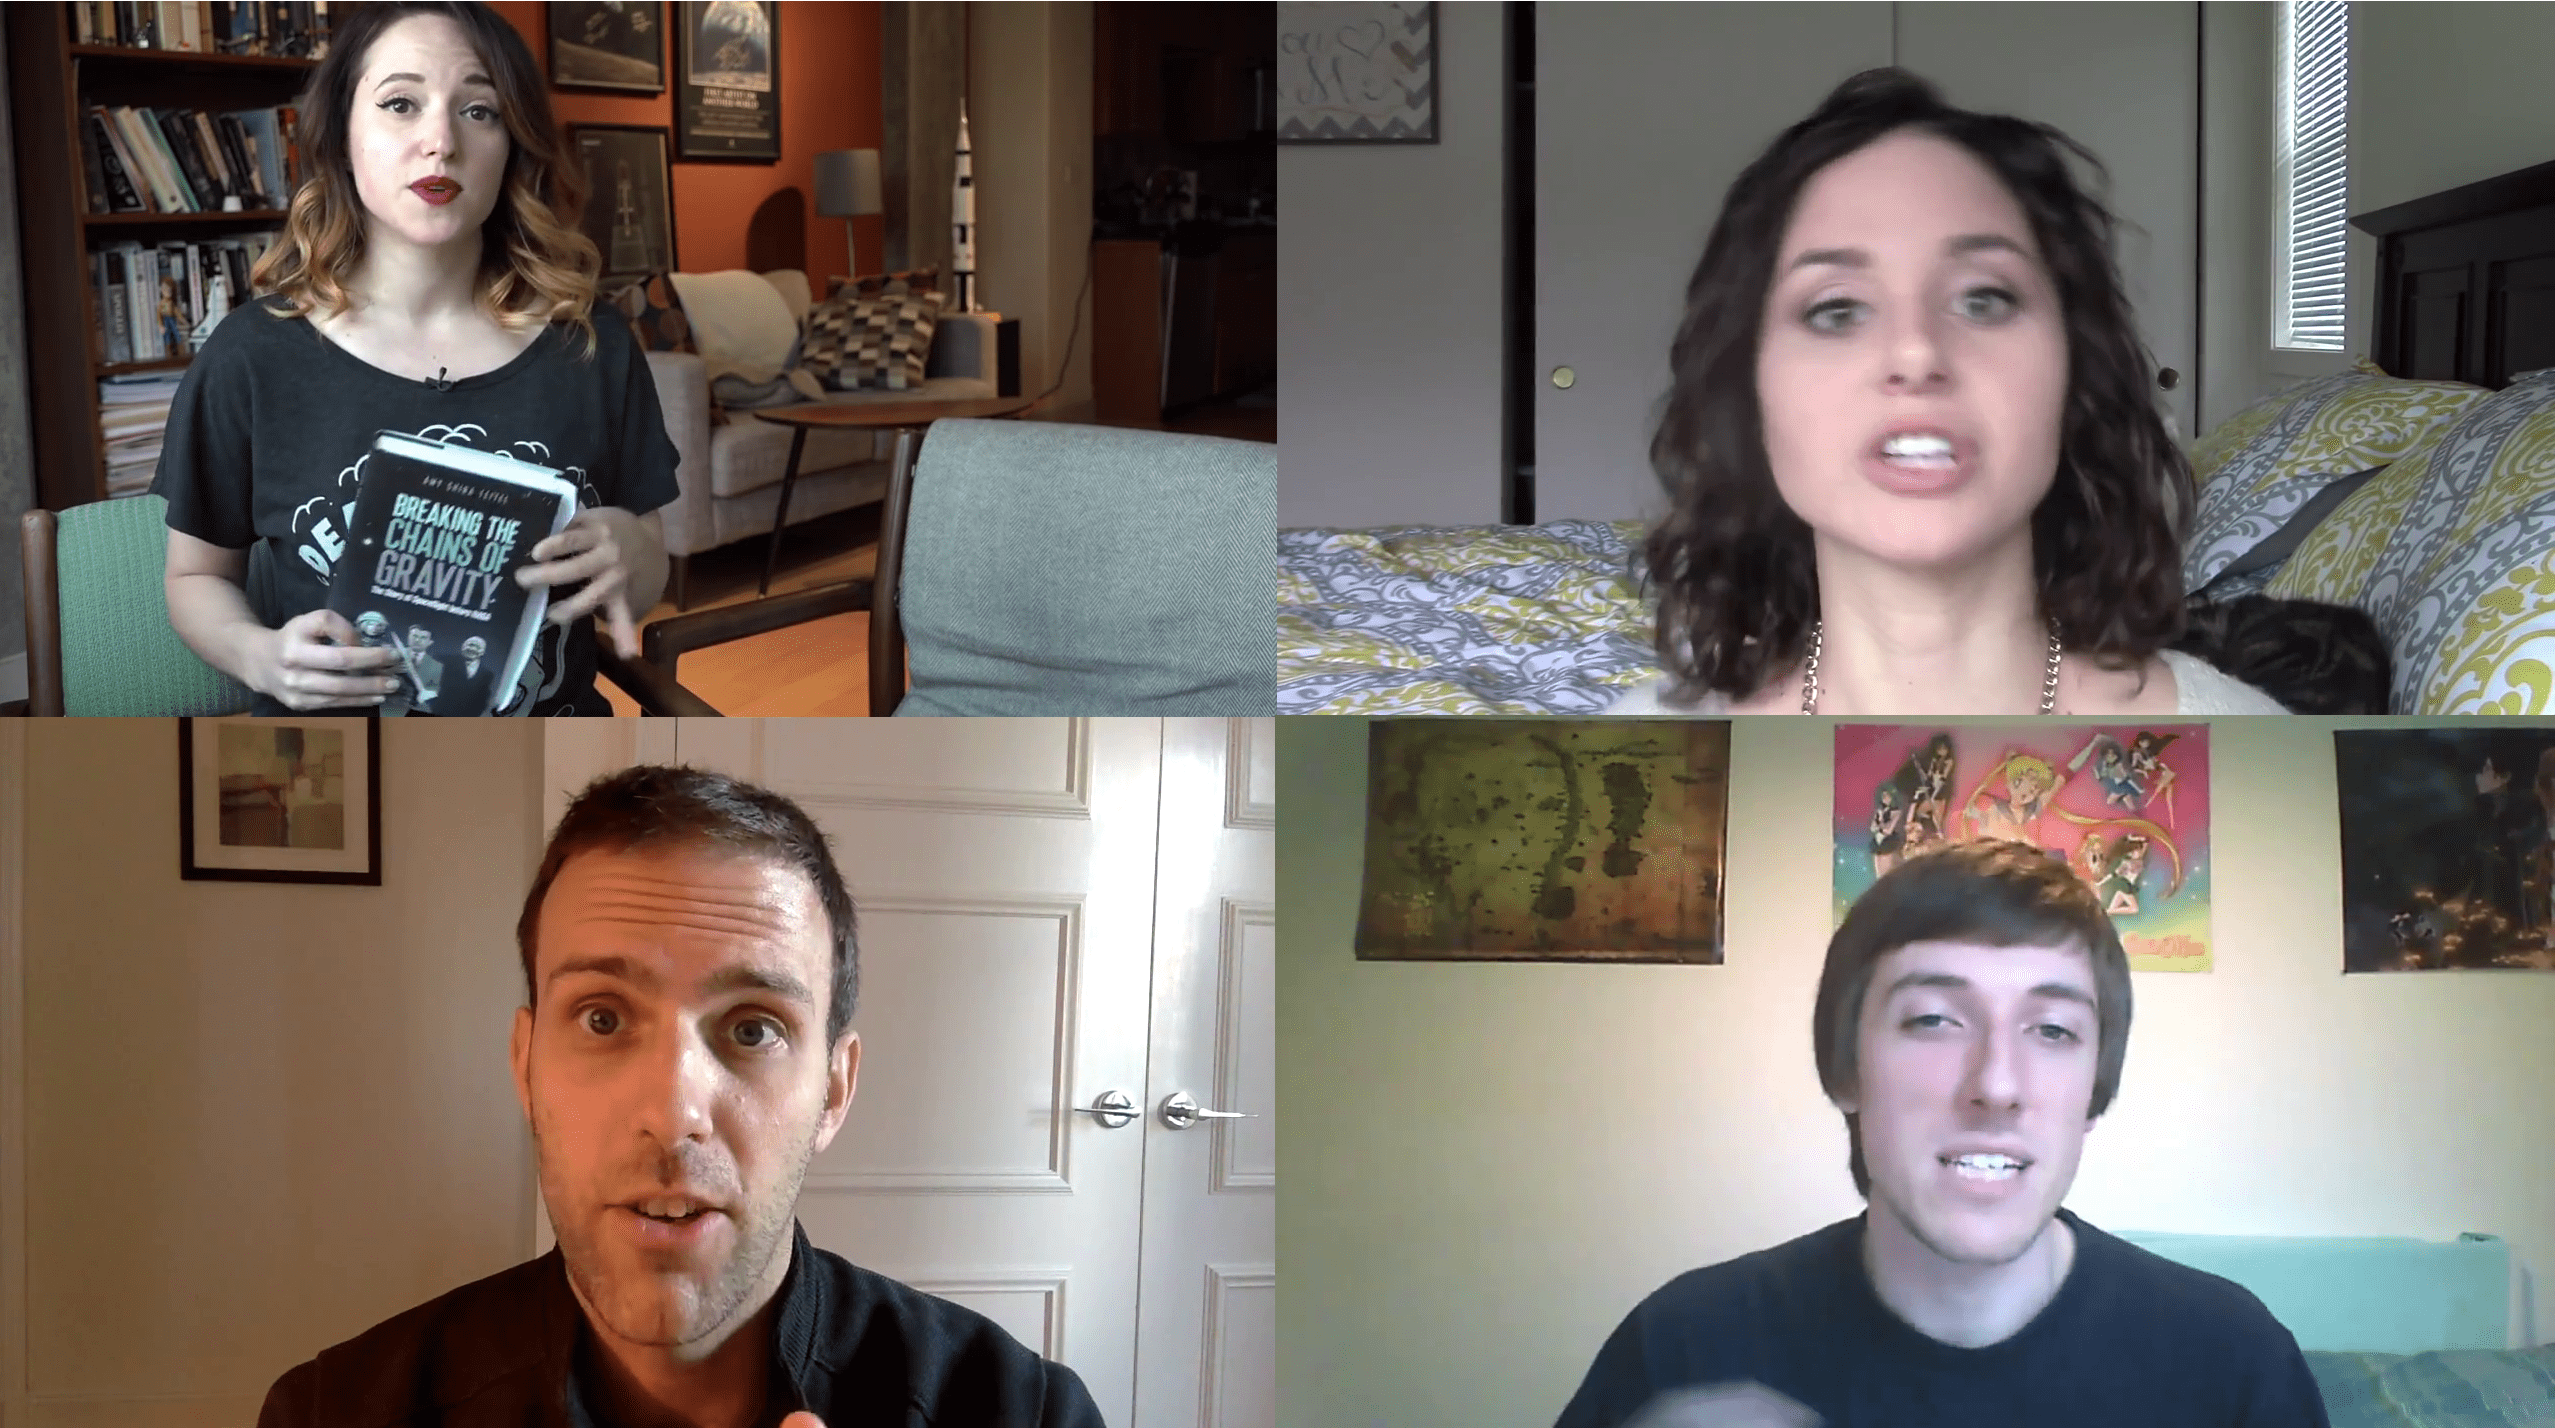
\includegraphics[width=0.8\textwidth]{Images/sample_video_clips-min.png}
  \caption{Screenshots from four samples of the video clip data-set.}
  \label{fig:ssvideoclip}
\end{figure*}


\subsection{Annotating Data}
\label{subsection:annotatingdata}
The selected 960 video clips were annotated additionally for mood primitives, likeability and a variable describing the presence of background music. The mood primitives, valence and arousal, and likeability were annotated with an ordinal scale with 3 classes. An annotation of class 1 means the variable scored low or negatively, class 2 is the neutral case, and class 3 means the variable scored high or positively. Initially the scale was set with 5 classes, however annotations with class 1 or class 5 were scarce so a smaller scale was chosen to improve the accuracy of the models. 

Two annotators annotated the same 960 video clips for these 4 dimensions. After which, the annotations were merged to create two additional data-sets. One data-set used the minimum of the two annotation, while the second one used the maximum of the two annotations. As a result, there were now 4 sets of annotations available to use and model classifiers with.

To measure the inter-rater reliability between the two annotators the Cohen's kappa coefficient was calculated. This coefficient is considered more robust as it takes into account the occurrence of an agreement by chance. The resulting coefficient will determine whether the agreement is accidental or not. Table \ref{tab:cohenkappa} shows the results of the Cohen's kappa calculations. The observed agreement (po) is the number of agreements divided by the total of number items. The random agreement (pe) is the probability that the annotators agreed on either of the possible annotations. Using the observed and random agreement the Cohen's kappa can be calculated. The coefficient ranges from 0 to 1 and can be interpreted as shown in Table \ref{tab:cohenkappainterpret}.

\begin{table*}[]
\begin{tabular}{|l|l|r|r|r|P{1.3cm}|P{2cm}|P{2cm}|}
\hline
\rowcolor{Gray}
\textbf{Dimension} & \textbf{Weight} & \multicolumn{1}{l|}{\textbf{po}} & \multicolumn{1}{l|}{\textbf{pe}} & \multicolumn{1}{l|}{\textbf{Kappa}} & \multicolumn{1}{l|}{\textbf{Kappa Error}} & \textbf{Agreement} & \textbf{Null hypothesis} \\ \hline
\multirow{3}{*}{\textbf{Arousal}} & Unweighted & 0.6229 & 0.4077 & 0.3634 & 0.0264 & Fair & Rejected \\ \cline{2-8} 
 & Linear & 0.8073 & 0.6713 & 0.4138 & 0.0387 & Moderate & Rejected \\ \cline{2-8} 
 & Quadratic & 0.8995 & 0.8031 & 0.4896 & 0.0493 & Moderate & Rejected \\ \hline
\multirow{3}{*}{\textbf{Valence}} & Unweighted & 0.7177 & 0.5046 & 0.4302 & 0.0293 & Moderate & Rejected \\ \cline{2-8} 
 & Linear & 0.8573 & 0.7371 & 0.4571 & 0.0429 & Moderate & Rejected \\ \cline{2-8} 
 & Quadratic & 0.9271 & 0.8534 & 0.5027 & 0.0572 & Moderate & Rejected \\ \hline
\multirow{3}{*}{\textbf{Likeability}} & Unweighted & 0.5812 & 0.4230 & 0.2743 & 0.0276 & Fair & Rejected \\ \cline{2-8} 
 & Linear & 0.7818 & 0.6704 & 0.3380 & 0.0404 & Fair & Rejected \\ \cline{2-8} 
 & Quadratic & 0.8820 & 0.7941 & 0.4272 & 0.0506 & Moderate & Rejected \\ \hline
\end{tabular}
\caption{Inter rater agreement results. po: observed agreement, pe: random agreement, Kappa: Cohen's Kappa.}
\label{tab:cohenkappa}
\end{table*}

\begin{table}[]
\begin{tabular}{|P{2cm}|P{4cm}|}
\hline
\rowcolor{Gray}
Cohen's Kappa & Agreement \\ \hline
0 & Agreement equivalent to chance \\ \hline
0.10 - 0.20 & Slight \\ \hline
0.21 - 0.40 & Fair \\ \hline
0.41 - 0.60 & Moderate \\ \hline
0.61 - 0.80 & Substantial \\ \hline
0.81 - 0.99 & Near perfect \\ \hline
1 & Perfect \\ \hline
\end{tabular}
\caption{Cohen's kappa agreement interpretation.}
\label{tab:cohenkappainterpret}
\end{table}

Since Cohen's kappa takes into account the disagreement but not the degree of disagreement a modified version of Cohen's kappa can be used which is the weighted Cohen's kappa (\cite{cohen1968weighted}). This can be applied well if an ordinal scale is used for the ratings. Since the annotations of the data-set use an ordinal scale, the weighted Cohen's kappa can be applied. The weighted kappa is calculated with the use of a table containing weights, which measures the degree of disagreement. This can be linear or quadratic. Table \ref{tab:cohenkappa} shows the results of the weighted Cohen's kappa alongside the unweighted versions. 

Overall, every dimension shows a moderate agreement when quadratic weighting is applied. Further, for every dimension and weight the null hypothesis is rejected, where the null hypothesis is that the observed agreement is accidental. Therefore it is safe to say the inter-rater reliability is higher than chance level. The data was then split up in a train set of 660 video clips and a test set of 300 video clips to be used for model training, optimization and testing. 

\subsection{Video Feature Extraction}\label{subsection:featureextraction}
To train our models we use video features that are extracted from the 15 second YouTube clips provided by the ChaLearn Competition. The features are facial features which are extracted over the entire video clip. These features are summarized by functionals. First, the faces were detected and then aligned using the Supervised Descent Method (\cite{xiong2013supervised}). Every detected face is rotated using the roll angle which is estimated from the eye corners. Also, there are 49 landmarks located on each face to which a 20\% margin is applied to corp the image to a size of 64 x 64 pixels. Image-level features are extracted from a convolutional neural network which was trained for emotion recognition (\cite{kaya2017video}). This network is a pre-trained VGG-Face network (\cite{parkhi2015deep}), which is optimized for large data-sets. The final layer of the network was changed to a 7-dimensional emotion recognition layer. The resulting network was then fine-tuned using the FER-2013 data-set (\cite{goodfellow2015challenges}), which contains over 35,000 images. The final trained network has 37 layers from which the 33rd response was used. This descriptor has 4096 dimensions which were then summarized using four statistical functions. Those functions were the mean, standard deviation, slope and offset from a linear polynomial.

\subsection{Feature Normalization}
\label{subsection:normalization}
Z normalization transforms the input vector into a vector where the mean is 0 or very close to 0 while the standard deviation is close to 1. The number for a single data point of the computed output vector can also be called the z-score. This score essentially is the number of standard deviations a vector is away from the mean. It can indicate how familiar a data point is relative to the others. 

\begin{figure*}[h]
  \centering
  \includesvg[width=\textwidth]{Images/featurenormalization_pipeline.svg}
  \caption{Feature normalization pipeline}
  \label{fig:normpipeline}
\end{figure*}

While Z normalization is applied at feature level L2 normalization is applied at feature vector level. L2 normalization is applied at each row of the feature set so that if the values are squared and then summed, they add up to exactly 1. 

Figure \ref{fig:normpipeline} shows the flowchart of the normalization steps that were applied at feature and vector level. 



\subsection{Classification Algorithms}
\label{subsection:classificaiton}
Several types of models were used for classification from the extracted video features. These models include:
\begin{enumerate}
\item Extreme Learning Machines (ELM)
\item Support Vector Machines (SVM)
\item Decision Trees (DT)
\item Ridge Classification
\end{enumerate}
In the first stage we use the ELM and SVM classifiers, while in the second stage we use the predictions of the ELM classifier to train a decision tree and linear model. The second stage classifications will give an indication of the feature importance and contribute to the explainability of our classification models. 

Originally proposed by Huang in 2004 (\cite{huang2004extreme}), the learning algorithm for Extreme Learning Machine uses single-hidden layer feedforward neural networks (SLFN). It chooses the nodes randomly and analytically determines the the output weights for the neural network. As a result, the training speed of this algorithm is noticeably fast. The technical details of the classifiers can be found in \cite{huang2004extreme} and \cite{huang2006extreme}. However, in this thesis we use Kernel ELM, where the first level transformation is done implicitly in the kernel space and the second layer weights (mapping the kernel matrix to outputs) are learned analytically using regularized least squares. We use a linear kernel which has a regularization coefficient. We optimize this coefficient during training and with threefold subject independent cross-validation of the training set. 

Just like ELM, the SVM algorithm is used for regression and classification. SVMs is a supervised learning method which is effective when the number of features is high or even higher than the number of samples. The algorithm finds the optimal separating hyperplane in a dimensional space of size N, where N is the number of features. It then uses the hyperplane to classify the data-points. To obtain the most accurate model the algorithm finds the hyperplane where the margins of the hyperplane are the largest. Just like the ELM algorithm a linear kernel is used and a regularization coefficient is optimized. 

The models that are trained using the ELM and SVM algorithms will create a set of predictions of the personality trait, mood and likeability dimensions. The predictions of the ELM classifier will be used in the second stage of our classification. During this stage, the predictions are stacked to a Decision Tree classifier as high level features. The DT classifier is trained using the predictions and the interview invitation variable as labels. Then, the trained DT can be visualized which contributes to the explainability and interpretability of our classification model.

Lastly, the same prediction data set to train the Decision Tree classifier is used to train a linear model. We will be using the Ridge Classifier which converts the target values to -1 and 1. Then, the model treats the problem as a regression problem. The trained model will provide us with the coefficient of the features of the decision function. In other words, the feature importance can be derived from these models which will show us what feature is the most or least important for determining the class.


